\documentclass[12pt,a4paper]{article}

\usepackage[a4paper, margin=1in]{geometry}
\usepackage{graphicx}
\usepackage{booktabs}
\usepackage{array}
\usepackage{longtable}
\usepackage{tabularx}
\usepackage{xcolor}
\usepackage{colortbl}
\usepackage{fancyhdr}
\usepackage{titlesec}
\usepackage{enumitem}
\usepackage{hyperref}
\usepackage[T1]{fontenc}
\usepackage[utf8]{inputenc}
\usepackage{parskip}
\usepackage{amsmath}
\setlength{\headheight}{14pt}
\usepackage{multirow}
\usepackage{makecell}
\usepackage{lastpage}
\usepackage{float}

\graphicspath{{images/}}

\definecolor{darkblue}{RGB}{31,56,100}
\definecolor{medblue}{RGB}{46,80,144}
\definecolor{tableheadbg}{RGB}{31,56,100}
\definecolor{rowaltbg}{RGB}{238,242,248}
\definecolor{hred}{RGB}{192,0,0}
\definecolor{mred}{RGB}{127,127,0}
\definecolor{gray}{RGB}{136,136,136}

\hypersetup{
    colorlinks=true,
    linkcolor=medblue,
    urlcolor=medblue,
    pdftitle={UML Models - Hotel Automation Software v1.0},
    pdfauthor={Project Team}
}

\titleformat{\section}
  {\Large\bfseries\color{darkblue}}
  {\thesection}{1em}{}
  [\vspace{2pt}\color{medblue}\titlerule[1pt]\vspace{4pt}]
\titleformat{\subsection}
  {\large\bfseries\color{medblue}}
  {\thesubsection}{1em}{}
\titleformat{\subsubsection}
  {\normalsize\bfseries\color{medblue}}
  {\thesubsubsection}{1em}{}

\pagestyle{fancy}
\fancyhf{}
\fancyhead[L]{\small\color{medblue} UML Models}
\fancyhead[R]{\small\color{gray} Hotel Automation Software}
\fancyfoot[L]{\small\color{gray} Version 1.0 \textbar\ Confidential}
\fancyfoot[R]{\small\color{gray} Page \thepage\ of \pageref{LastPage}}
\renewcommand{\headrulewidth}{0.5pt}
\renewcommand{\footrulewidth}{0.5pt}

\newcolumntype{L}[1]{>{\raggedright\arraybackslash}p{#1}}
\newcolumntype{C}[1]{>{\centering\arraybackslash}p{#1}}
\newcolumntype{R}[1]{>{\raggedleft\arraybackslash}p{#1}}

\renewcommand{\thead}[1]{%
  \cellcolor{tableheadbg}\color{white}\textbf{#1}%
}

\begin{document}

\thispagestyle{empty}
\begin{center}
  \vspace*{3cm}
  {\Huge\bfseries\color{darkblue} UML MODELS}\\[1em]
  {\LARGE\color{medblue} Hotel Automation Software}\\[3cm]

  \begin{tabular}{|L{4cm}|L{8cm}|}
    \hline
    \rowcolor{tableheadbg}
    \color{white}\textbf{Document Type} & \color{white} UML Analysis \& Design Models \\
    \hline
    \rowcolor{rowaltbg}
    \textbf{Subject}           & Software Engineering \\
    \hline
    \rowcolor{rowaltbg}
    \textbf{Subject Code}      & CS3004 \\
    \hline
    \textbf{Version}           & 1.0 (PlantUML-rendered diagrams) \\
    \hline
    \rowcolor{rowaltbg}
    \textbf{Date}              & \today \\
    \hline
    \rowcolor{rowaltbg}
    \textbf{Based on}          & SRS v1.0, SA/SD v1.0 \\
    \hline
    \textbf{Group Members}     &
      \begin{tabular}[t]{@{}L{4cm} L{3.5cm}@{}}
        Suyash Pandey        & : 2023UG1100 \\[3pt]
        Suraj Kumar          & : 2023UG1106 \\[3pt]
        Himanshu Raj          & : 2023UG1092 \\[3pt]
        Satyendra Kumar         & : 2023UG1105 \\
      \end{tabular} \\
    \hline
    \rowcolor{rowaltbg}
    \textbf{Institution}       & Indian Institute of Information Technology Ranchi, Jharkhand \\
    \hline
  \end{tabular}
\end{center}
\vfill

\newpage

\thispagestyle{fancy}
\tableofcontents
\newpage

% ══════════════════════════════════════════════════════════════════════════════
\section{Introduction}

This document presents the UML analysis and design models for the Hotel Automation
Software, derived from the SRS (v1.0) and the SA/SD document (v1.0). It contains:

\begin{itemize}[leftmargin=1.5em]
  \item A \textbf{use case diagram} capturing the user-observable behaviour.
  \item A \textbf{class diagram} showing the domain and controller classes, their
        attributes, operations, and relationships.
  \item \textbf{Sequence diagrams} for the three load-bearing runtime scenarios.
  \item \textbf{State-chart diagrams} for the Reservation, Room, and
        HotelController state machines.
\end{itemize}

\subsection*{Diagram toolchain}

Diagrams are authored in \textbf{PlantUML} (source in the \texttt{puml/} folder) and
rendered to PNG via the PlantUML online editor (\url{https://www.plantuml.com/plantuml})
or a local \texttt{plantuml.jar}. The PNG outputs live in \texttt{images/} and are
embedded below via \verb|\includegraphics|. See \texttt{UML/README.md} for full
rendering instructions.

Notation follows UML~2.5.

\newpage

% ══════════════════════════════════════════════════════════════════════════════
\section{Use Case Diagram}

\subsection{Actors}

The system has four actors corresponding to the user classes defined in SRS~\S2.3:
\begin{itemize}[leftmargin=1.5em]
  \item \textbf{Hotel Manager} (primary) --- configures rooms, tariffs, food menu, and
        discount policies; reviews occupancy reports.
  \item \textbf{Receptionist} (primary) --- manages guest reservations, room allocations,
        token issuance, and check-out.
  \item \textbf{Catering Services Manager} (primary) --- records food and beverage orders
        against guest token numbers.
  \item \textbf{Guest} (secondary) --- the indirect beneficiary; interacts with the
        system via the Receptionist and Catering Services Manager.
\end{itemize}

\subsection{Diagram}

\begin{figure}[H]
\centering
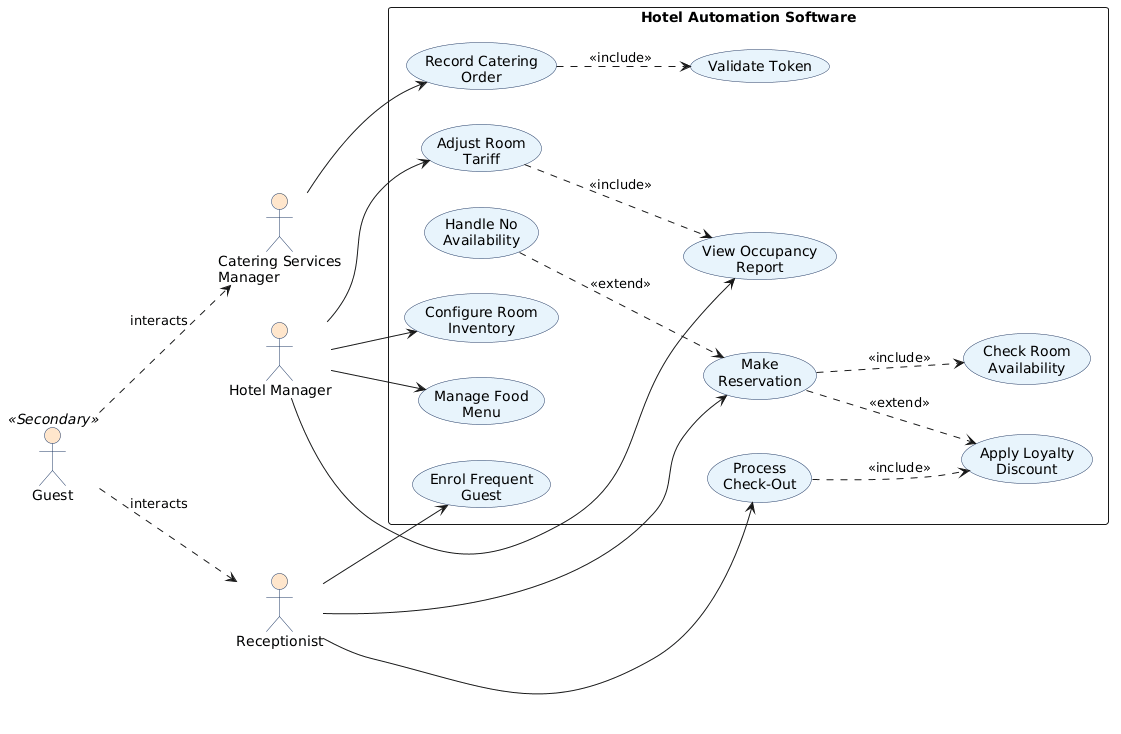
\includegraphics[width=0.95\textwidth,keepaspectratio]{usecase.png}
\caption{Use Case Diagram. Dashed arrows labelled
\textit{\textless{}include\textgreater{}} / \textit{\textless{}extend\textgreater{}}
indicate the corresponding UML relationships.}
\label{fig:usecase}
\end{figure}

\subsection{Use Case Summaries}

\begin{longtable}{|L{3.5cm}|L{9cm}|L{2.2cm}|}
  \hline
  \thead{Use Case} & \thead{Summary} & \thead{SRS Ref} \\
  \hline
  \endhead
  \hline
  \endfoot
  \rowcolor{rowaltbg}
  Make Reservation
    & Receptionist enters guest name, arrival date/time, duration, room type, advance
      payment, and optional loyalty ID. Includes \emph{Check Room Availability}.
      Extends with \emph{Apply Loyalty Discount} if identity number is provided.
    & FR-3.*, FR-4.* \\
  \hline
  Check Room Availability
    & Query room inventory for the requested type and date range; return lowest-numbered
      available room or a NoRoomAvailable flag.
    & FR-4.1, NFR-R3 \\
  \hline
  \rowcolor{rowaltbg}
  Handle No Availability
    & Extension of Make Reservation when no suitable room exists --- compose and
      display an apology message to the Receptionist.
    & FR-4.3 \\
  \hline
  Record Catering Order
    & Catering Services Manager enters token number, food item, quantity, and
      date/time. Includes \emph{Validate Token}.
    & FR-5.1--5.4 \\
  \hline
  \rowcolor{rowaltbg}
  Process Check-Out
    & Receptionist enters token number; system computes room and catering charges,
      applies advance deduction and optional loyalty discount, generates and prints
      the itemised bill, and marks the room available.
    & FR-6.1--6.6 \\
  \hline
  Apply Loyalty Discount
    & Included in Process Check-Out when a frequent-guest identity number is present
      --- look up discount percentage and reduce the total bill accordingly.
    & FR-7.2, FR-7.3 \\
  \hline
  \rowcolor{rowaltbg}
  Enrol Frequent Guest
    & Receptionist enrols a qualifying guest at check-out; system generates and
      issues a new loyalty identity number effective from the next stay.
    & FR-7.1, FR-7.4 \\
  \hline
  Adjust Room Tariff
    & Hotel Manager selects a room type and specifies a percentage adjustment;
      system computes the new tariff and logs the change. Includes
      \emph{View Occupancy Report}.
    & FR-2.2, FR-2.3 \\
  \hline
  \rowcolor{rowaltbg}
  View Occupancy Report
    & Hotel Manager selects a month; system computes and displays the average
      occupancy rate.
    & FR-2.1 \\
  \hline
  Configure Room Inventory
    & Hotel Manager defines room numbers, bed types, AC types, and base tariffs.
    & FR-1.1--1.3 \\
  \hline
  \rowcolor{rowaltbg}
  Manage Food Menu
    & Hotel Manager adds or updates food items and their unit prices.
    & FR-5.3 \\
  \hline
\end{longtable}

\newpage

% ══════════════════════════════════════════════════════════════════════════════
\section{Class Diagram}

\subsection{Overview}

The class model is organised into three logical layers:
\textbf{UI / Controller} (\texttt{HotelController}),
\textbf{Application core} (\texttt{DispatchTransaction}, \texttt{ProcessReservation},
\texttt{ProcessCheckOut}, \texttt{RecordCateringOrder}, \texttt{AdjustTariff},
\texttt{ViewOccupancy}, \texttt{ManageFrequentGuest}, \texttt{DBAccessLayer}),
and \textbf{Domain} (\texttt{Room}, \texttt{RoomType}, \texttt{Tariff},
\texttt{Reservation}, \texttt{CateringOrder}, \texttt{MenuItem},
\texttt{FrequentGuest}, \texttt{Bill}).

\subsection{Diagram}

\begin{figure}[H]
\centering
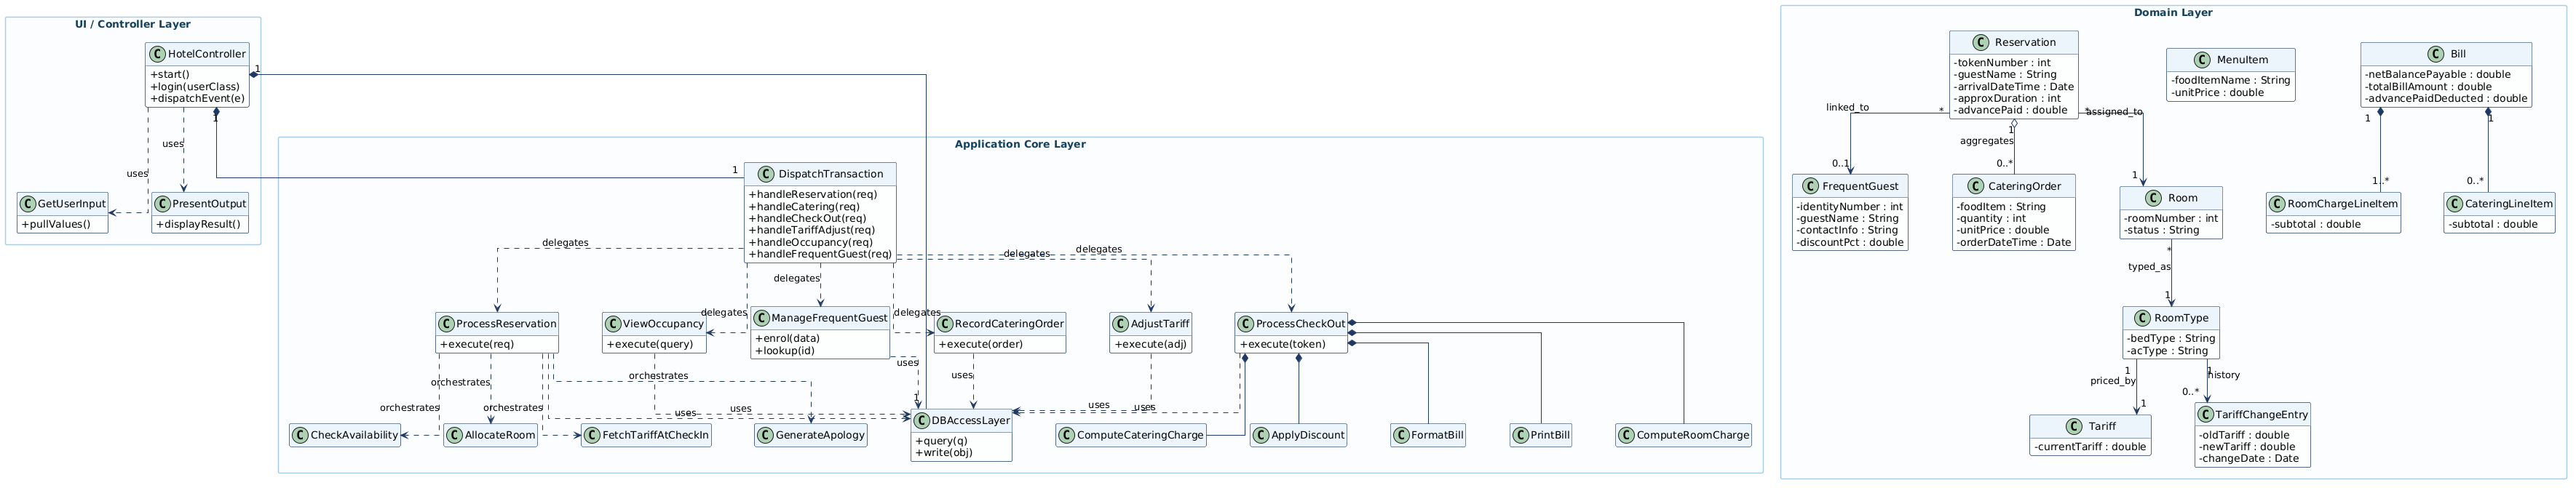
\includegraphics[width=\textwidth,keepaspectratio]{class.png}
\caption{Class Diagram. Filled diamonds: composition; open diamonds: aggregation;
open triangles: inheritance; plain arrows: association; dashed arrows: dependency.}
\label{fig:class}
\end{figure}

\subsection{Key Relationships}

\begin{itemize}[leftmargin=1.5em]
  \item \texttt{HotelController} composes \texttt{DispatchTransaction} and
        \texttt{DBAccessLayer}; it also uses \texttt{GetUserInput} and
        \texttt{PresentOutput} for UI mediation.
  \item \texttt{DispatchTransaction} delegates to \texttt{ProcessReservation},
        \texttt{ProcessCheckOut}, \texttt{RecordCateringOrder}, \texttt{AdjustTariff},
        \texttt{ViewOccupancy}, and \texttt{ManageFrequentGuest}.
  \item \texttt{ProcessReservation} orchestrates \texttt{CheckAvailability},
        \texttt{AllocateRoom}, \texttt{FetchTariffAtCheckIn}, and
        \texttt{GenerateApology}.
  \item \texttt{ProcessCheckOut} composes \texttt{ComputeRoomCharge},
        \texttt{ComputeCateringCharge}, \texttt{ApplyDiscount}, \texttt{FormatBill},
        and \texttt{PrintBill}.
  \item Every \texttt{Room} references one \texttt{RoomType}; each \texttt{RoomType}
        references one current \texttt{Tariff} and an ordered list of
        \texttt{TariffChangeEntry} objects.
  \item \texttt{Reservation} associates with one \texttt{Room} and optionally one
        \texttt{FrequentGuest}; it aggregates zero or more \texttt{CateringOrder}
        objects for billing.
  \item \texttt{Bill} is composed of one or more \texttt{RoomChargeLineItem} and
        zero or more \texttt{CateringLineItem} objects.
\end{itemize}

\newpage

% ══════════════════════════════════════════════════════════════════════════════
\section{Sequence Diagrams}

The three scenarios below exercise the load-bearing paths of the reservation and
billing workflows and together cover every transition in the Reservation and Room
state machines.

\subsection{Scenario A --- Successful Room Reservation (Walk-In or Advance)}

\begin{figure}[H]
\centering
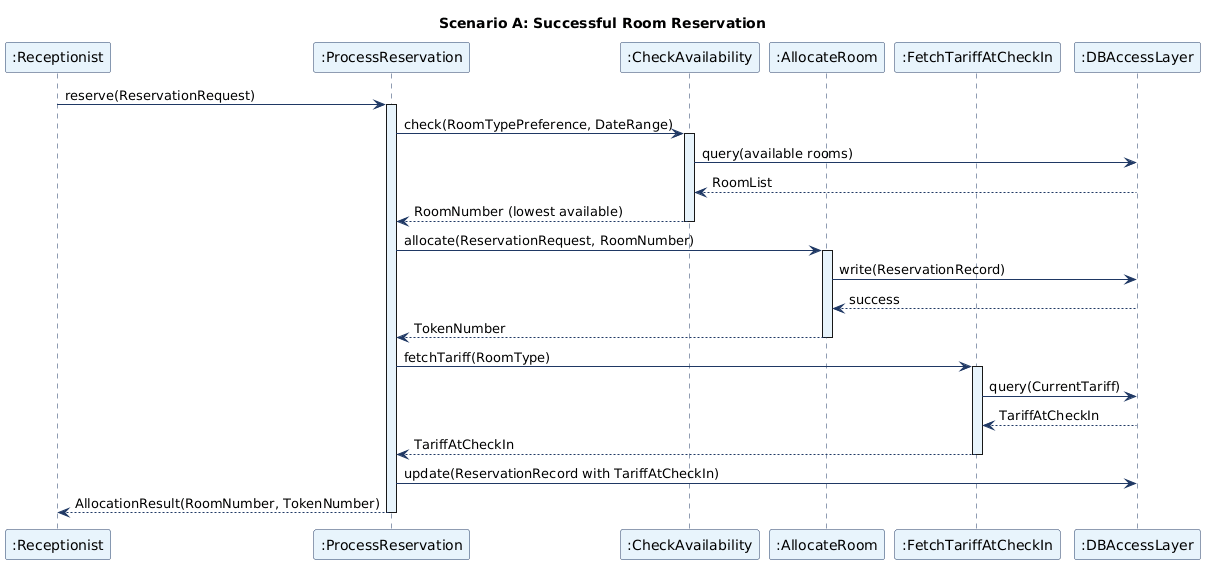
\includegraphics[width=0.95\textwidth,keepaspectratio]{sequence_A.png}
\caption{Scenario A. Receptionist submits a reservation request; a matching room is
available --- system allocates the room, issues a token number, and fetches the
tariff at check-in time. (FR-3.1, FR-4.1, FR-4.2, FR-4.4, FR-6.2)}
\label{fig:seqA}
\end{figure}

\subsection{Scenario B --- Reservation Rejected (No Suitable Room)}

\begin{figure}[H]
\centering
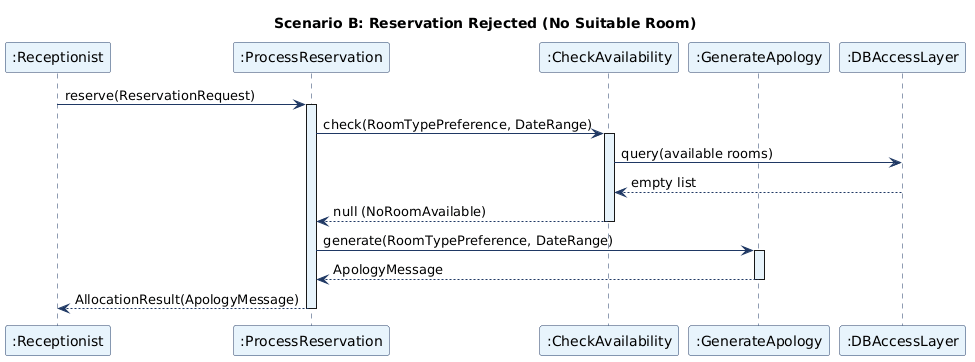
\includegraphics[width=0.9\textwidth,keepaspectratio]{sequence_B.png}
\caption{Scenario B. Reservation request is submitted but no room of the requested
type is available for the requested dates --- system generates and returns an apology
message. (FR-4.1, FR-4.3)}
\label{fig:seqB}
\end{figure}

\subsection{Scenario C --- Guest Check-Out with Frequent-Guest Discount}

\begin{figure}[H]
\centering
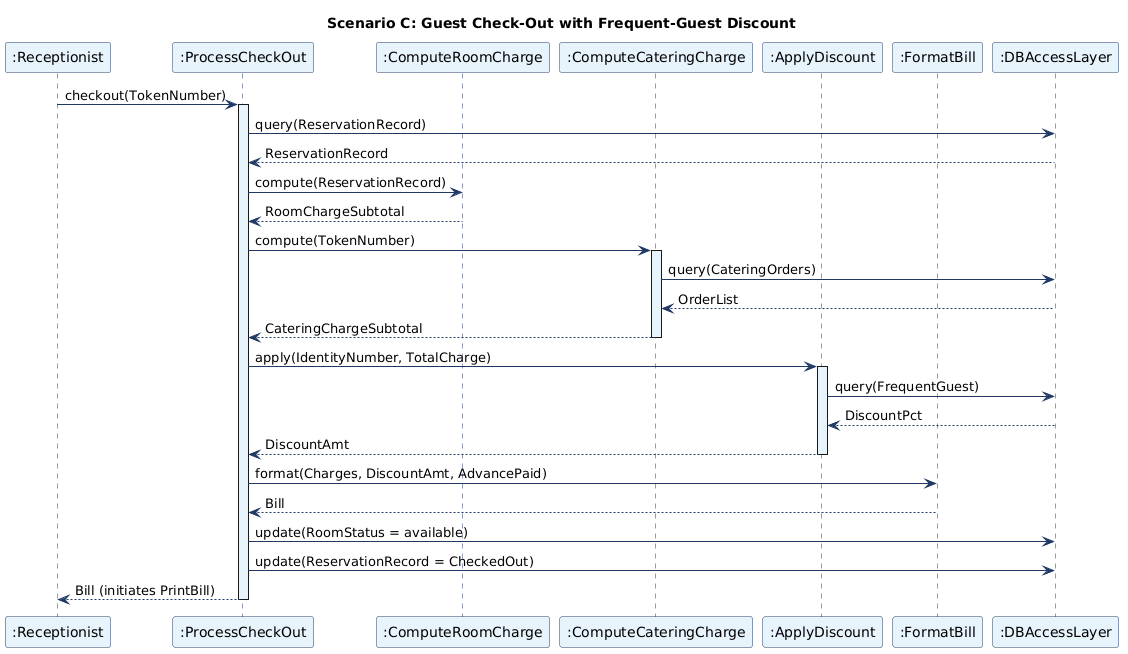
\includegraphics[width=\textwidth,keepaspectratio]{sequence_C.png}
\caption{Scenario C. Receptionist initiates check-out; system retrieves reservation
and catering records, computes room and catering charges, applies the frequent-guest
discount, formats the itemised bill, and marks the room available.
(FR-6.1--6.6, FR-7.2--7.3)}
\label{fig:seqC}
\end{figure}

\newpage

% ══════════════════════════════════════════════════════════════════════════════
\section{State-Chart Diagrams}

\subsection{Room State-Chart}

\begin{figure}[H]
\centering
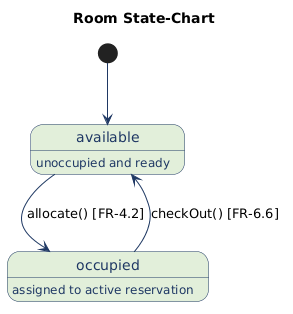
\includegraphics[width=0.7\textwidth,keepaspectratio]{state_room.png}
\caption{Room state-chart. Two states correspond to FR-1.3's availability partition.
Transitions are triggered by successful allocation (FR-4.2) and check-out completion
(FR-6.6).}
\label{fig:stateRoom}
\end{figure}

\subsection{Reservation State-Chart}

\begin{figure}[H]
\centering
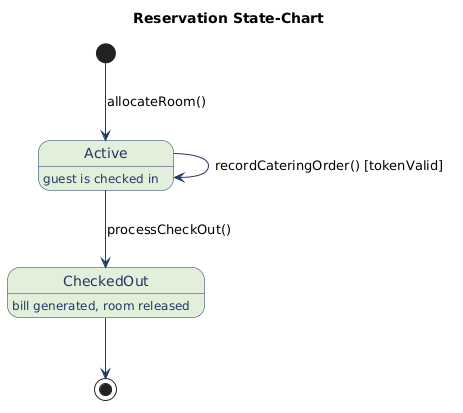
\includegraphics[width=0.75\textwidth,keepaspectratio]{state_reservation.png}
\caption{Reservation state-chart. The \texttt{[tokenValid]} guard reflects FR-5.2's
active-guest check used by the catering module. The \texttt{[checkedOut]} transition
triggers bill generation and room release. (FR-3.*, FR-4.*, FR-6.1, FR-6.6)}
\label{fig:stateReservation}
\end{figure}

\subsection{HotelController State-Chart}

\begin{figure}[H]
\centering
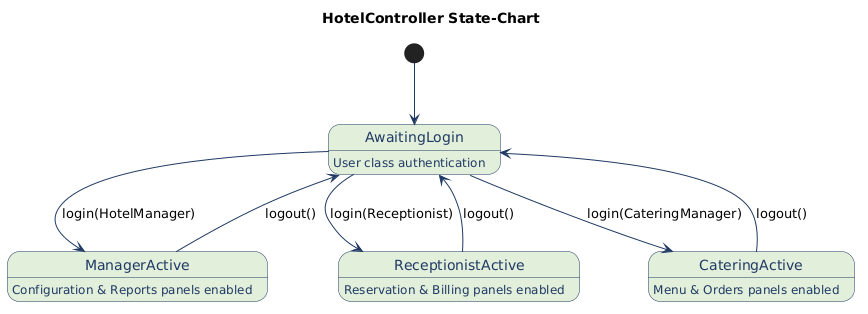
\includegraphics[width=0.85\textwidth,keepaspectratio]{state_controller.png}
\caption{HotelController state-chart covering the GUI lifecycle and role-based
panel activation. (FR-8.1, NFR-S1)}
\label{fig:stateCtrl}
\end{figure}

\newpage

% ══════════════════════════════════════════════════════════════════════════════
\section{Traceability --- UML to SRS}

\begin{longtable}{|L{5cm}|L{3.5cm}|L{5cm}|}
  \hline
  \thead{UML Artefact} & \thead{Figure} & \thead{Primary SRS Ref} \\
  \hline
  \endhead
  \hline
  \endfoot
  \rowcolor{rowaltbg}
  Use Case: Configure Room Inventory   & Fig.~\ref{fig:usecase}           & FR-1.1--1.3 \\
  \hline
  Use Case: Adjust Room Tariff         & Fig.~\ref{fig:usecase}           & FR-2.2, FR-2.3 \\
  \hline
  \rowcolor{rowaltbg}
  Use Case: View Occupancy Report      & Fig.~\ref{fig:usecase}           & FR-2.1 \\
  \hline
  Use Case: Make Reservation           & Fig.~\ref{fig:usecase}           & FR-3.*, FR-4.* \\
  \hline
  \rowcolor{rowaltbg}
  Use Case: Handle No Availability     & Fig.~\ref{fig:usecase}           & FR-4.3 \\
  \hline
  Use Case: Record Catering Order      & Fig.~\ref{fig:usecase}           & FR-5.1--5.4 \\
  \hline
  \rowcolor{rowaltbg}
  Use Case: Process Check-Out          & Fig.~\ref{fig:usecase}           & FR-6.1--6.6 \\
  \hline
  Use Case: Apply Loyalty Discount     & Fig.~\ref{fig:usecase}           & FR-7.2, FR-7.3 \\
  \hline
  \rowcolor{rowaltbg}
  Use Case: Enrol Frequent Guest       & Fig.~\ref{fig:usecase}           & FR-7.1, FR-7.4 \\
  \hline
  Class: HotelController               & Fig.~\ref{fig:class}             & FR-8.1, NFR-S1 \\
  \hline
  \rowcolor{rowaltbg}
  Class: ProcessReservation            & Fig.~\ref{fig:class}             & FR-3.*, FR-4.* \\
  \hline
  Class: ProcessCheckOut               & Fig.~\ref{fig:class}             & FR-6.1--6.6, FR-7.2--7.3 \\
  \hline
  \rowcolor{rowaltbg}
  Class: RecordCateringOrder           & Fig.~\ref{fig:class}             & FR-5.1--5.4 \\
  \hline
  Class: ManageFrequentGuest           & Fig.~\ref{fig:class}             & FR-7.1--7.4 \\
  \hline
  \rowcolor{rowaltbg}
  Class: DBAccessLayer                 & Fig.~\ref{fig:class}             & NFR-R5 \\
  \hline
  Class: Room, RoomType, Tariff        & Fig.~\ref{fig:class}             & FR-1.*, FR-2.* \\
  \hline
  \rowcolor{rowaltbg}
  Class: Reservation, CateringOrder    & Fig.~\ref{fig:class}             & FR-3.*, FR-4.*, FR-5.* \\
  \hline
  Class: Bill                          & Fig.~\ref{fig:class}             & FR-6.4, NFR-R4 \\
  \hline
  \rowcolor{rowaltbg}
  Class: FrequentGuest                 & Fig.~\ref{fig:class}             & FR-7.1--7.4 \\
  \hline
  Sequence A (reservation $\to$ alloc) & Fig.~\ref{fig:seqA}              & FR-3.1, FR-4.1, FR-4.2, FR-6.2 \\
  \hline
  \rowcolor{rowaltbg}
  Sequence B (reservation $\to$ apology)& Fig.~\ref{fig:seqB}             & FR-4.1, FR-4.3 \\
  \hline
  Sequence C (check-out $\to$ bill)    & Fig.~\ref{fig:seqC}              & FR-6.1--6.6, FR-7.2, FR-7.3 \\
  \hline
  \rowcolor{rowaltbg}
  State-chart: Room                    & Fig.~\ref{fig:stateRoom}         & FR-1.3, FR-4.2, FR-6.6 \\
  \hline
  State-chart: Reservation             & Fig.~\ref{fig:stateReservation}  & FR-3.*, FR-4.*, FR-5.2, FR-6.1, FR-6.6 \\
  \hline
  \rowcolor{rowaltbg}
  State-chart: HotelController         & Fig.~\ref{fig:stateCtrl}         & FR-8.1, NFR-S1 \\
  \hline
\end{longtable}

% ══════════════════════════════════════════════════════════════════════════════
\section{Revision History}

\begin{longtable}{|L{2cm}|L{3cm}|L{4cm}|L{4.5cm}|}
  \hline
  \thead{Version} & \thead{Date} & \thead{Author} & \thead{Description} \\
  \hline
  \endhead
  \hline
  \endfoot
  \rowcolor{rowaltbg}
  1.0 & \today & Project Team
    & Initial UML models for Hotel Automation Software. Use case diagram (11 use
      cases, 4 actors), class diagram (three-layer architecture), sequence diagrams
      for Scenarios A--C, and state-chart diagrams for Room, Reservation, and
      HotelController. Authored in PlantUML (\texttt{puml/}), rendered to PNG, and
      embedded via \texttt{\textbackslash includegraphics}. All SRS cross-references
      included. \\
  \hline
\end{longtable}

\vfill
\begin{center}
  \color{medblue}\rule{0.6\linewidth}{0.5pt}\\[0.5em]
  \color{gray}\small\textit{End of Document --- Hotel Automation Software UML v1.0}
\end{center}

\end{document}